\documentclass{article}
\usepackage[utf8]{inputenc}
\usepackage{graphicx}
\usepackage{xcolor}
\usepackage{romana}
\usepackage{url}

\begin{document}


\title{\textbf{
\includegraphics[scale=0.5]{Sigla_Ucv.png}
\textcolor{blue}{Universitatea din Craiova \\Facultatea de Automatic'a, Calculatoare 'si Electronic'a}}}
\date{\today}

\maketitle

\begin{center}

\includegraphics[scale=0.72]{Tortul_Regelui}
\end{center}
\textbf{Student : Nedianu Gabriel-C'at'alin} \\
\textbf{Specializarea: Calculatoare Rom"an'a\\ Anul I\\ Grupa: CR 1.2 B}

\newpage

\tableofcontents

\newpage

\newpage

\section{Enun\c{t}ul Problemei}


\emph {Tortul 'Imp'aratului Ro'su} \\

'Imp'aratul Ro'su a comandat pentru nunta fiului s'au un tort 'imp'ar'atesc cu n straturi 
circulare. Buc'atarii 'imp'aratului au preg'atit tortul pe un platou de argint. 'Ins'a, 'imp'aratul dore'ste ca tortul s'a fie mutat pe un platou de aur. Din cauza dimensiunii enorme a tortului, opera'tia de transfer trebuie realizat'a cu mare aten'tie, pentru a evita distrugerea accidental'a a tortului; a'sa c'a buc'atarii nu 'stiu cum s'a mute tortul de pe platoul de argint pe platoul de aur. Ei 'si-au dat 'insa seama c'a, pentru mutarea tortului, pot folosi un al treilea platou de bronz. La fiecare pas este cel mai sigur s'a transfere un singur strat al tortului de pe un platou pe altul 'si 'intotdeauna un strat al tortului va fi pus doar peste un strat de diametru mai mare, astfel 'incat s'a se evite deteriorarea tortului. Scrie'ti un program care s'a ajute buc'atarii s'a transfere tortul f'ar'a s'a 'il strice, astfel 'inc"at tortul transferat s'a fie identic cu tortul ini'tial.
Se vor implementa doi algoritmi diferi'ti.

\section{Algoritmii}

\subsection{Algoritmul 1 (recursiv)}
\begin{center}
\begin{tabbing}

MUTA\_TORTUL($numar\_felii, platou\_initial, platou\_final, platou\_ajutator$)\\
1.\indent{\bf daca} \= ($numar\_felii == 1$) \\
2.\indent           \>{\bf afiseaza} Se muta stratul 1 al tortului de pe $platou\_initial$ pe $platou\_final$\\ 
3.\indent{\bf altfel}\= \\
4.\indent           \>MUTA\_TORTUL($numar\_felii-1, platou\_initial, platou\_ajutator, platou\_final$) \\
5.\indent           \>{\bf afiseaza}  Se muta stratul 1 al tortului de pe $platou\_initial$ pe $platou\_ajutator$\\ 6.\indent           \>MUTA\_TORTUL($numar\_felii-1, platou\_ajutator, platou\_final, platou\_initial$) \\
\end{tabbing}
\end{center}

Complexitatea de timp a algoritmului este O($2^n$), deoarece fiecare func'tie se va reapela de alte dou'a ori pana c"and se va ajunge ca numar\_felii primit de func'tie s'a fie 1. 'In total vor fi: $2^1+2^2+...+2^{n-1}$ reapel'ari + apelarea ini'tiala:$2^0$.

Complexitatea de memorie a algoritmului este O($n$), deoarece recursivitatea nu va fi mai mare pe o ramur'a de $n$ ori.

Algoritmul func'tioneaz'a astfel: se consider'a c'a tortul format din n straturi va fi a'sezat ini'tial pe primul platou (cel de argint) 'si se dore'ste ca acesta s'a fie mutat pe platoul final (cel de aur) cu ajutorul platoului ajut'ator (cel de bronz).
Consider'am c'a toate straturile tortului, f'ar'a ultimul, se vor muta pe platoul ajut'ator, apoi ultimul strat va fi mutat pe platoul final; la final, straturile aflate pe platoul ajut'ator se vor muta pe ultimul platoul peste ultimul strat.

\newpage

{\Large Schema recursivit'a'tii primului algoritm}

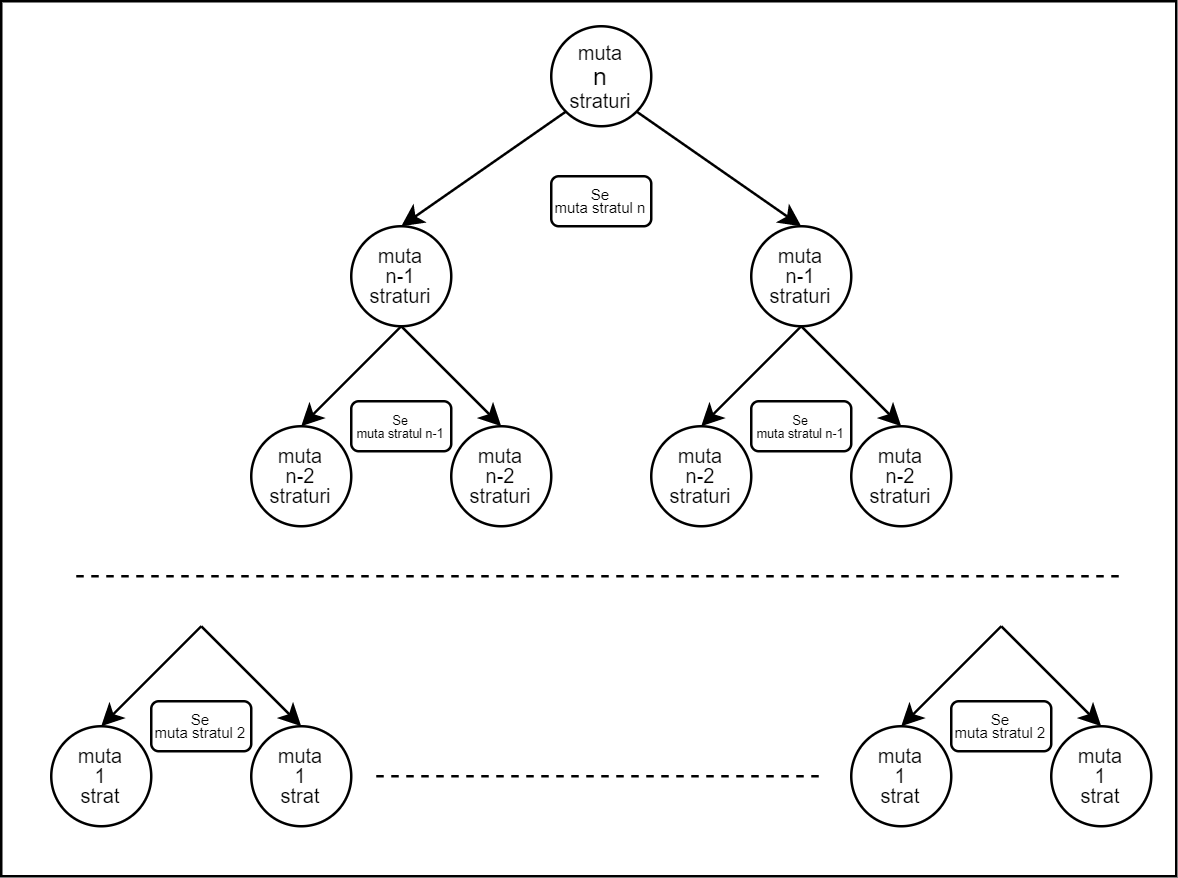
\includegraphics[scale=0.3]{DiagramaRecursivitateaALG1}\\

\subsection{Algoritmul 2 (iterativ)}

\begin{center}
\begin{tabbing}

Muta\_Tortul\_Iterativ($nr\_straturi$,$*platou\_initial$,$*platou\_final$,$*platou\_ajutator$) \\
1.\indent{\bf daca} \=($nr\_straturi\%2==0$) \\
2.\indent           \>interschimba($platou\_final-nume,platou\_ajutator-nume$)\\
3.\indent creeaza\_tortul($*platou\_intial,nr\_straturi$)\\
4.\indent $nr\_mutarii = 0$\\
4.\indent{\bf cat timp} \=(este\_plin($*platou\_final$) $!= 1$ $\&\&$ este\_plin($*platou\_ajutator$)   $!=1$) \\
5.\indent               \>$nr\_mutarii++$ \\
6.\indent               \>{\bf daca} \=($numarul\_mutarii \% 3 == 1$)\\
7.\indent               \>           \>muta\_strat\_intre($*platou\_initial$,$*platou\_final$)\\
8.\indent               \>{\bf daca} \=($numarul\_mutarii \% 3 == 2$)\\
7.\indent               \>           \>muta\_strat\_intre($*platou\_initial$,$*platou\_ajutator$)\\
8.\indent               \>{\bf altfel}\\
9.\indent               \>           \>muta\_strat\_intre($*platou\_ajutator$,$*platou\_final$)\\


\end{tabbing}
\end{center}

Pentru acest algoritm am folosit o structur'a, *platou, care va fi folosit'a ca o stiv'a pentru a stoca straturile aflate pe fiecare platou, 'in ordine.

Complexitatea de timp a acestui algoritm depinde de num'arul de mut'ari efectuate, experiment"and aceasta ajunge s'a fie O($2^n$).

Complexitatea de memorie este O($n$), deoarece se vor utiliza doar trei vectori de capacitate maxim'a n pentru a stoca straturile 'si se va lucra doar cu ace'stia.


Algoritmul func'tioneaz'a astfel (pentru torturile cu numar de straturi impar): dac'a se mut'a consecutiv c"ate un strat 'intre dou'a platouri, se va ajunge ca tortul s'a fie mutat complet pe un alt platou. Ordinea de mutare a straturilor este urm'atoarea: se mut'a 'intre primul 'si ultimul platou stratul posibil, se mut'a 'intre primul 'si al doilea platou stratul posibil, apoi se mut'a 'intre cel de-al doilea 'si cel de-al treilea platou stratul posibil.
Aceste mut'ari se vor repeta p"an'a c"and tortul va fi mutat complet pe al treilea platou (cel de aur).

'In cazul torturilor cu num'ar de straturi par, principiul este acela'si, singura diferen't'a fiind c'a se schimb'a pu'tin ordinea mut'arilor: prima mutare va fi 'intre primul platou 'si cel de-al doilea, a doua mutare 'intre primul platou 'si ultimul platou, iar cea de-a treia 'intre cel de-al doilea 'si cel de-al treilea platou. Astfel, va trebui s'a fie inversat platoul final cu cel ajut'ator ca s'a ramana mut'arile de la cazul cu num'ar de straturi impare (lucru ce se poate face schimb"and doar denumirile acestora, av"and 'in vedere c'a stivele sunt goale).

Deci, se vor face serii de c"ate trei mut'ari consecutive, aceste mut'ari acoperind toate mi's'carile posibile 'intre cele trei platouri.

Pentru a verifica corectitudinea num'arului de pa'si, am introdus variabila numarul\_mutarii, care va ar'ata la final c'a'ti pa'si vor fi necesari pentru mutarea tortului.

Itera'tia va func'tiona p"an'a c"and tortul va fi mutat pe platoul final necesar, 'si astfel se va afla 'si numarul mut'arilor necesare.
\begin{center}
Schema celui de-al doilea algoritm pentru un tort cu dou'a 'si trei straturi\\
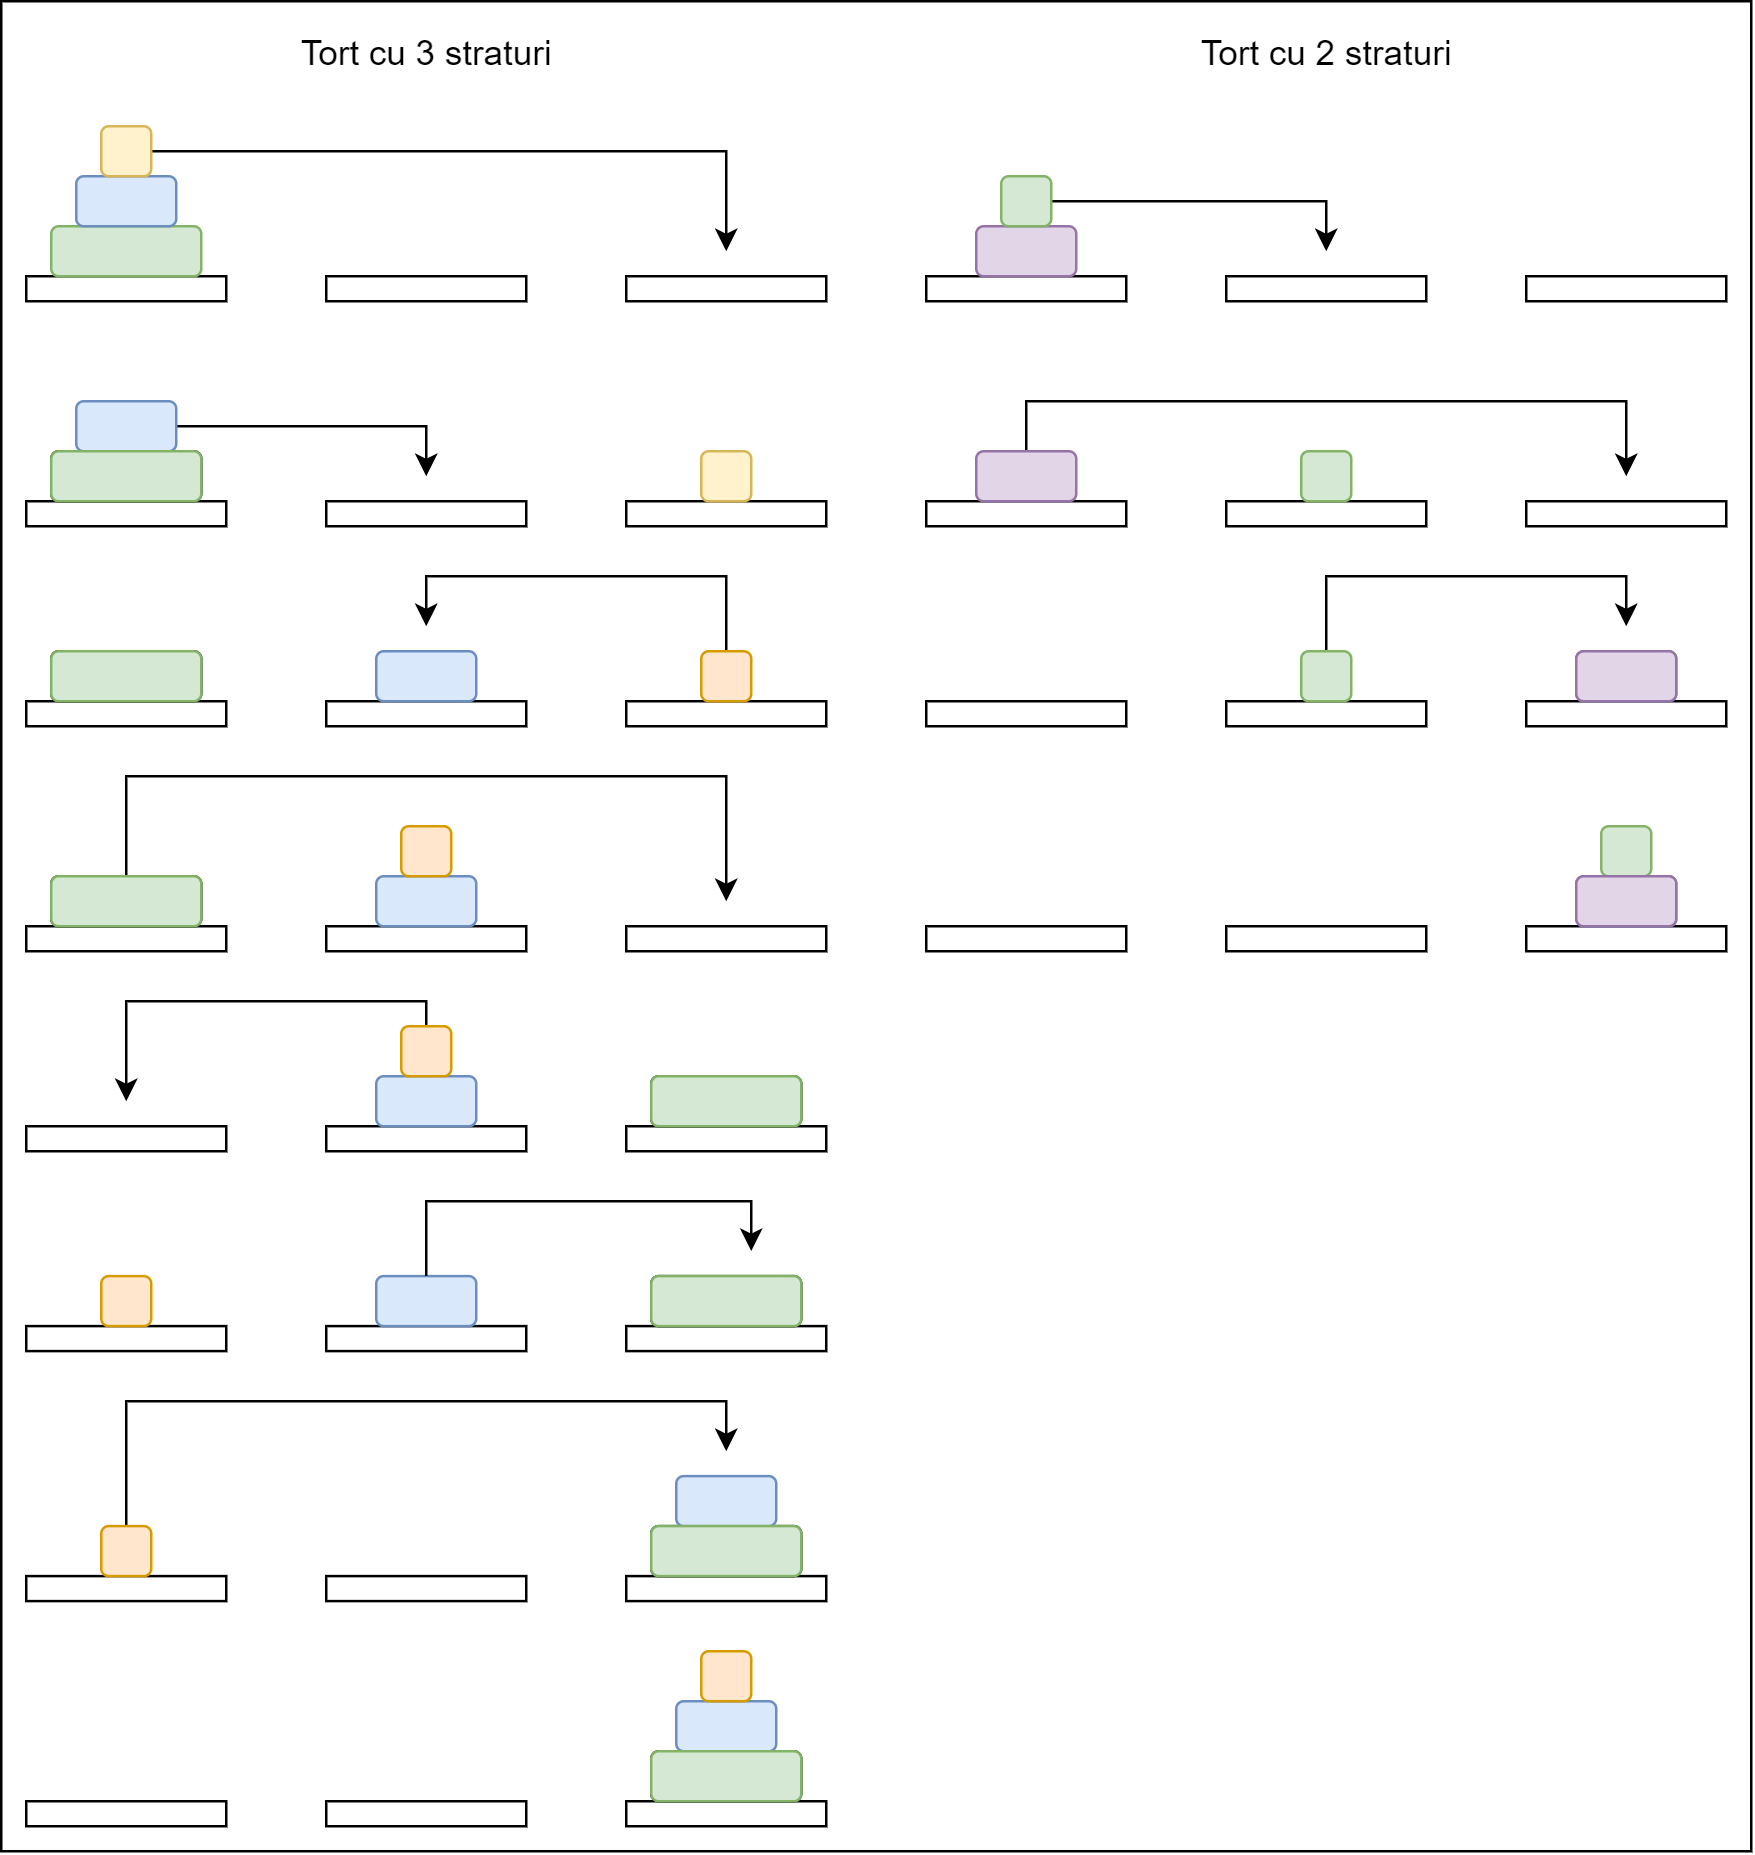
\includegraphics[scale=0.123]{Algoritm_Iterativ}\\
\end{center}

\section{Date Experimentale}

Ca date de intrare, problema are nevoie de un singur parametru, acela fiind num'arul de straturi pe care 'il va avea tortul, care urmeaz'a a fi mutat de pe platoul de argint pe cel de aur.

'In prima etap'a a cre'arii programului, datele de intrare apar'tineau intervalului $(1,23)$, iar pentru salvarea pa'silor mut'arii tortului 'in fi'sier, se ocupa un spa'tiu mai mare de 500 Mb (pentru 23 de straturi) 'si executarea programului dureaz'a peste 50 de secunde cu oricare dintre algoritmi.

Dup'a ce am limitat numarul de pa'si scri'si la 1000, am putut m'ari intervalul pana la 31, 'in acest caz execu'tia dur"and maxim 50-60 secunde, 'in cel mai r'au caz (31 de straturi), iar fi'sierul de output are doar 60 Kb.

Am creat un generator simplu care va genera un num'ar din intervalul $(1,31)$ folosind, 'in limbajul C func'tia rand(), iar 'in limbajul Python o func'tie asem'an'atoare, randitnd().


\section{Proiectarea aplica\c{t}iei experimentale}

\subsection{Structura de nivel 'inalt a aplica'tiei}

Aplica'tia con'tine urm'atoarele fi'siere 'in limbajul C: main.c, tort.c, torth.h, generator\_nr\_straturi.c, generator\_nr\_straturi.h conectate astfel:

\begin{center}
    
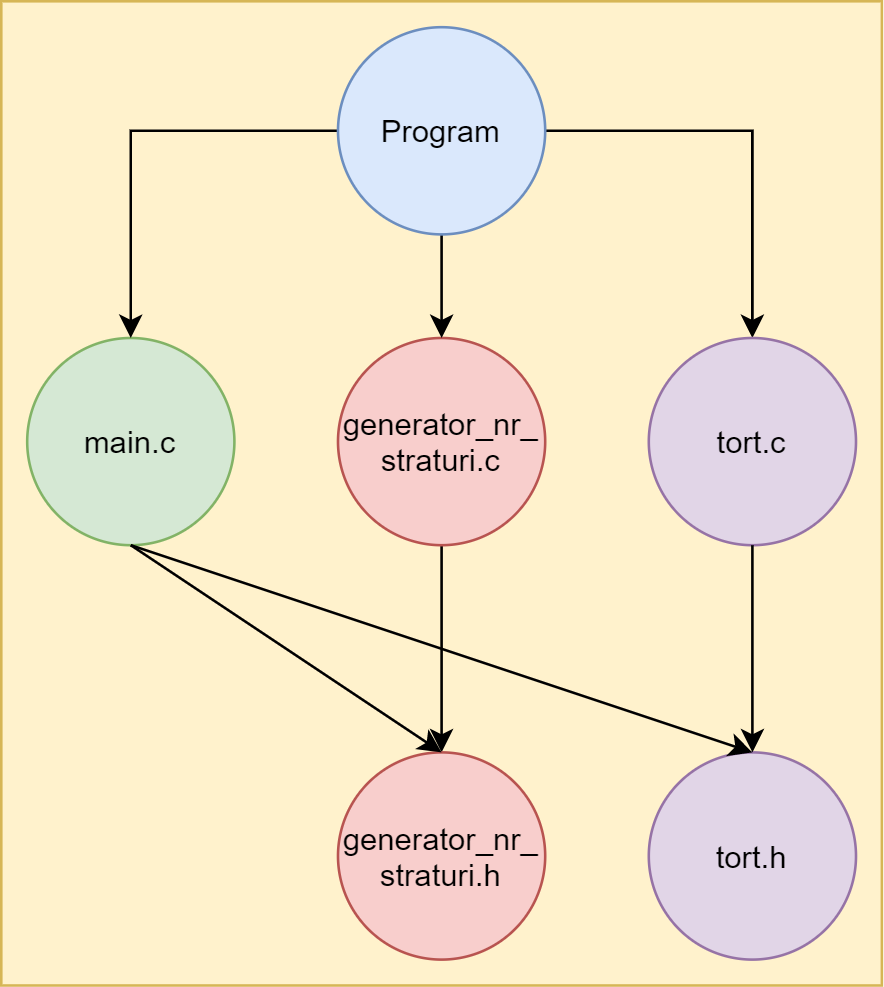
\includegraphics[scale=0.24]{StructuraPeNivelInaltC}\\

\end{center}
\newpage


Aplica'tia con'tine urm'atoarele fi'siere 'in limbajul Python: Tort\_Principal.py, Tort\_Func.py si Generator\_Straturi\_Tort.py conectate astfel:

\begin{center}
    
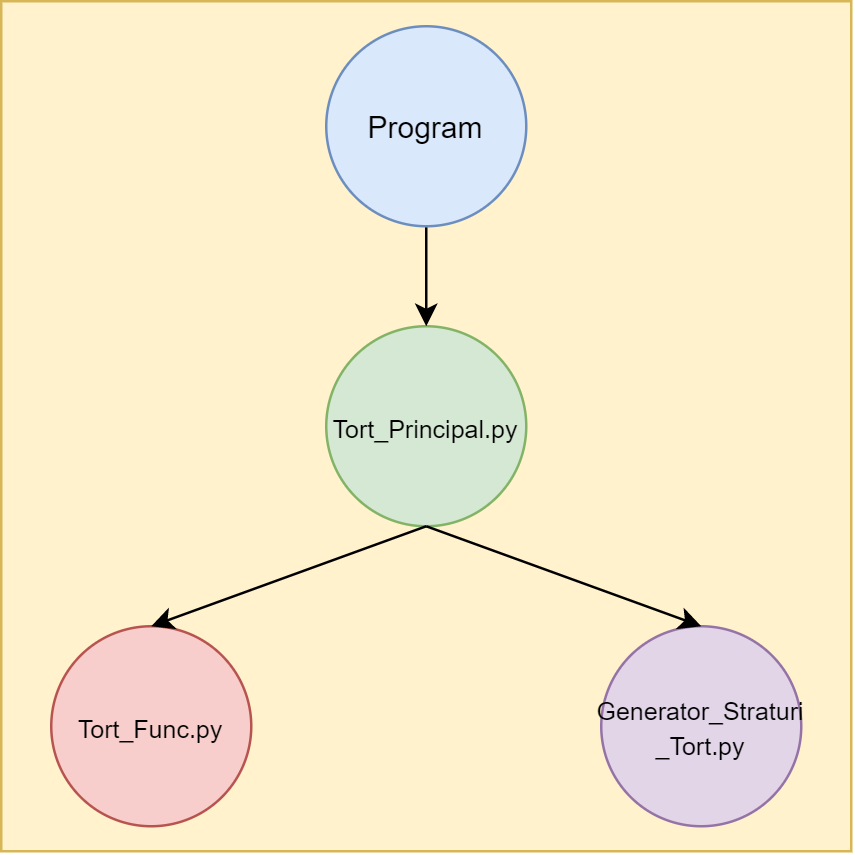
\includegraphics[scale=0.25]{StructuraPeNivelInaltPY}\\

\end{center}

\subsection{Descrierea Mul'timii Datelor de intrare}

Singura dat'a de intrare pentru algoritm va fi un num'ar, care va simboliza num'arul de straturi ale tortului ce urmeaz'a s'a fie mutat.

\subsection{Descrierea Mul'timii Datelor de ie'sire}

Datele de ie'sire ale problemei vor fi stocate 'in mod implicit 'intr-un fisier .txt numit ajutor\_bucatari ('in timpul testelor, aceste date vor fi stocate 'in fi'siere test\_i, i fiind cuprinse 'intre 1 'si 10). \\

Fi'sierul de ie'sire va cuprinde pe primul r"and un mesaj ini'tial, care va ar'ata c"ate straturi are tortul, pe urm'atoarele r'anduri pa'sii ce trebuie f'acu'ti pentru a muta tortul de pe platoul ini'tial pe cel final (pa'sii care vor fi afisa'ti sunt limita'ti la 1000), pe penultimul r"and va fi un mesaj ce va ar'ata num'arul de mut'ari necesare pentru a muta tortul, iar pe ultimul r"and va fi afi'sat timpul de execu'tie ('in secunde).

\newpage

\subsection{Lista modulelor aplica'tiei}

{\large In C , modulele sunt:}

\begin{itemize}

    \item main.c                    -modulul principal
    \item tort.c                    -modulul ce cuprinde majoritatea corpurilor func'tiilor utilizate
    \item generator\_nr\_straturi.c -modulul 'in care se afl'a corpul func'tiei, care va genera automat num'arul de straturi 
    \item tort.h - modulul ce con'tine headerele func'tiilor din tort.c
    \item generator\_nr\_straturi.h modulul ce con'tine headerele func'tiei de generare
    
\end{itemize}
{\large In Python , modulele sunt:}

\begin{itemize}
    \item Tort\_Principal.py -modulul principal
    \item Tort\_Func.py -modulul 'in care sunt scrise majoritatea func'tiilor
    \item Generator\_Straturi\_Tort.py -modulul care con'tine generatorul

\end{itemize}

\subsection{Func'tiile aplica'tiei}
\subsubsection{main.c}
Pentru ambii algoritmi, acest modul con'tine doar deschiderea fi'sierelor unde se vor salva datele, apeluri de func'tii, ini'tializ'ari de structuri necesare/variabile 'si metoda prin care este cronometrat timpul de execu'tie al algoritmului.   \\

Pentru algoritmul recursiv, 'in main.c sunt apelate func'tiile \\
\textcolor{blue}{genereaza\_straturi\_tort()} 'si \textcolor{green}{muta\_tortul()}. \\ 

Pentru algoritmul iterativ 'in main.c sunt apelate func'tiile \\
\textcolor{blue}{genereaza\_straturi\_tort()}, \textcolor{brown}{creeaza\_platou()} 'si \textcolor{purple}{muta\_tortul()}.\\

Pentru ambii algoritmi poate fi apelat'a 'si func'tia \textcolor{red}{test()}, ce a fost folosit'a pentru a efectua testele.

Testarea timpului a fost efectuat'a utiliz"andu-se libr'aria <time.h> 'si func'tia clock().

\subsubsection{generator\_nr\_straturi.h si tort.h}

Aici se afl'a prototipurile func'tiilor folosite 'si o variabil'a global'a nr\_straturi\_tort.
Pentru algoritmul iterativ, tot aici (tort.h) se va g'asi declara'tia structurii Platou, ce va fi o stiv'a 'in care se vor stoca straturile tortului aflate pe un anumit platou, dar 'si numele platoului.\\
Pentru algoritmul recursiv, aici se va g'asi o variabil'a global'a, 'in care se va salva num'arul de mut'ari necesare.

\subsubsection{generator\_nr\_straturi.c}

'In acest modul se g'ase'ste corpul func'tiei ce genereaz'a aleatoriu un num'ar de straturi al torului din intervalul (1,31): \textcolor{blue}{genereaza\_straturi\_tort()}. Aceast'a func'tie nu returneaz'a nimic, deoarece schimb'a automat valoarea variabilei globale nr\_straturi.
Sunt folosite func'tiile srand() 'si rand().


\subsubsection{tort.c}

Aici se g'asesc corpurile majorit'a'tii func'tiilor folosite 'in programe.\\

Pentru algoritmul recursiv g'asim doar func'tia \textcolor{green}{muta\_tortul()}. Aceast'a func'tie prime'ste ca parametrii: num'arul de straturi ale tortului, numele celor trei platouri 'si pointerul la fi'sierul 'in care se vor salva informa'tiile.
Aceasta este func'tia principal'a care creeaz'a recursivitatea prin care se mut'a \\straturile tortului, recursivitate explicat'a 'in \textbf{Sec'tiunea 2.1}
Func'tia nu returneaz'a nimic, aceasta scrie 'in fi'sierul ajutor buc'atari pa'sii/mut'arile necesare care vor fi limitate de variabila definit'a ca limita\_afisari = 1000; dupa ce se trece de aceast'a limit'a, recursiunea se va realiza f'ar'a afi'sare.\\

Tot 'in acest modul, 'in ambele file ale ambilor algoritmi, vom folosi func'tia \textcolor{red}{test()}, ce va ajuta la efectuarea testelor pentru ni'ste valori prestabilite, prin care se va testa func'tionalitatea programului, timpul de execu'tie 'si num'arul de pa'si ce vor fi efectua'ti pentru fiecare test 'in parte. Algoritmul va fi testat pentru urm'atoarele straturi de tort : 1, 3, 6, 14, 15, 20, 21, 27, 30, 31.\\


Pentru algoritmul iterativ, aici se g'asesc mai multe func'tii folosite. \\
Majoritatea func'tiilor sunt folosite utiliz"and structura Platou creat'a \\
Structura Platou este o stiv'a ce va con'tine num'arul de straturi ale tortului 'in timpul mut'arii acestora. Aceasta are 'in componen'ta sa nr\_straturi\_maxime, un vector de tip char ce va con'tine numele platoului respectiv, variabila top ce va reprezenta c"ate straturi se afl'a 'in acel moment pe platou (-1 reprezint'a faptul c'a platoul este gol) 'si un vector de tip int ce va stoca num'arul straturilor aflate pe platou, 'in ordinea asez'arii lor.

Func'tia \textcolor{brown}{creeaza\_platou()} creeaz'a platoul propriu-zis.

Func'tia \textcolor{red}{este\_plin()} prime'ste ca parametru un Platou 'si returneaz'a dac'a acesta este plin sau nu. Pentru a afla dac'a platoul este plin, am verificat dac'a straturile maxime admise de un platou sunt egale cu num'arul de elemente aflate 'in el (deoarece numerotarea straturilor 'incepe de la 0, am sc'azut 1 din num'arul de straturi maxime).

Func'tia \textcolor{red}{nu\_sunt\_straturi()} func'tioneaz'a asem'an'ator cu func'tia anterioar'a, diferen'ta fiind c'a aceasta verific'a dac'a nu sunt straturi ale tortului pe platou.

Func'tia \textcolor{red}{adauga()} prime'ste ca parametrii un Platou 'si o variabila de tip int ce reprezinta num'arul stratului ce va fi ad'augat pe platoul respectiv. Valoarea top a platoului este crescut'a cu 1.

\newpage

Func'tia \textcolor{red}{scoate\_stratul()} prime'ste un Platou, returneaz'a ultimul strat aflat pe acesta 'si este sc'azut'a valoarea top a platoului cu -1. Dac'a nu sunt straturi pe acel platou, este returnat'a valoarea "-2".

Func'tia \textcolor{red}{muta\_strat\_salvare()} prime'ste num'arul stratului ce se va muta, numele platourilor 'intre care se va face mutarea 'si un pointer la fi'sierul 'in care va fi salvat'a aceast'a mutare.

Func'tia  \textcolor{red}{creaza\_tortul()} prime'ste un Platou 'si adaug'a pe acesta straturile tortului de la cel mai mare la cel mai mic. Astfel, ultimul strat ad'augat va fi scos primul.
Aceast'a func'tie va fi folosit'a pentru a pune tortul pe platoul ini'tial.

Functia  \textcolor{red}{muta\_straturile\_intre\_2\_platouri()} prime'ste dou'a Platouri 'si pointer la fi'sierul de output; aceast'a func'tie va muta ultimul strat mai mic dintre cele dou'a platouri peste stratul mai mare.\\
Aceast'a func'tie scoate ultimul strat din fiecare platou 'si compar'a aceste straturi, exist"and patru cazuri posibile.
Primul caz este acela 'in care primul platou este gol; astfel, se va muta stratul de sus al celui de-al doilea platou peste acesta 'si se va salva mutarea. Al doilea caz este cel 'in care cel de-al doilea platou are stratul superior gol. 'In ultimele dou'a cazuri se compar'a straturile superioare ale celor dou'a platouri, stratul mai mare se adaug'a la loc pe platoul de unde provine, iar cel'alalt se asaz'a peste el 'si apoi se savleaz'a mutarea in fi'sier.

Func'tia \textcolor{red}{muta\_straturile\_intre\_2\_platouri\_fara\_afisare()} func'tioneaza identic cu func'tia anterioar'a, doar c'a nu se mai salveaz'a (sau afi'seaz'a) mut'arile .

Func'tia \textcolor{purple}{muta\_tortul()} prime'ste ca parametrii num'arul de straturi ale tortului, cele trei structuri reprezent"and fiecare platou 'si fisierul de output.\\
Prima parte a func'tiei va schimba denumirea platoului ajut'ator cu cea al celui final, dac'a avem un num'ar par de straturi.\\
'In urm'atoarea parte a func'tiei se va crea tortul pe primul platou (adaug"and straturile de la cel mai mare la cel mai mic pe acesta).\\
'In ultima parte a func'tiei va 'incepe itera'tia prin care se mut'a strat cu strat tortul, dupa tiparul definit 'in \textbf{Sec'tiunea 2.2}. Avem o instruc'tiune while, 'in care se vor num'ara mut'arile efectuate p"an'a c"and tortul va fi complet mutat.

\subsubsection{Tort\_Principal.py}

Acesta este modulul principal al func'tiei 'in Phyton, pentru ambii algoritmi; aici doar vom apela func'tii 'si vom ini'tializa variabilele pentru testarea timpului.

Variabilele 'si func'tiile au denumiri aproximativ asem'an'atoare cu cele din C, iar func'tionalitatea lor este aceea'si.

Tot aici va fi apelat'a o func'tie nou'a, \textcolor{red}{afisare\_nr\_pasi()}, care va salva 'in fi'sier num'arul de pa'si efectua'ti de buc'atari pentru a muta tortul, aceast'a func'tie primind doar pointerul la fi'sier.

'In acest modul vom avea 'si modalitatea de testare (ce a fost comentat'a pentru a permite rularea o singur'a dat'a a programului, f'ar'a a rula 'si testul).

\newpage

\subsubsection{Generator\_Straturi\_Tort.py}

'In acest modul avem func'tia care genereaz'a straturile tortului pentru rul'ari la 'int"amplare, fiind creat'a folosind func'tia random redenumit'a r, ce ne va returna un numar din intervalul (1, 31).\\
Aici am creat 'si variabila nr\_straturi\_tort 'in care, la fiecare rulare, se va salva alt num'ar format de generator.


\subsubsection{Tort\_Func.py}
 
'In acest modul vom g'asi func'tiile folosite pentru ambii algoritmi din ambele programe 'in Phyton, dar 'si variabila limita\_afisari ce va limita num'arul de afi's'ari 'in fiecare program la 1000.\\

Pentru algoritmul recursiv, avem funct'iile: 

Func'tia \textcolor{green}{muta\_tortul()}, func'tia principal'a, care va fi folosit'a pentru a salva 'in fi'sier mut'arile ce vor fi efectuate de buc'atari (am folosit func'tia globals() pentru a salva printr-o itera'tie 'si num'arul de pa'si ce va fi afi'sat la final 'si va fi folosit ca o verificare), aceast'a func'tie primind num'arul de straturi, denumirile celor trei platouri 'si fi'sierul de output. Modul de func'tionare al algoritmului a fost explicat anterior.

Func'tia \textcolor{red}{afisare\_numar\_pasi()} func'tie ce prime'ste fi'sierul de output 'si salveaz'a 'in el penultima linie, con'tin"and un mesaj cu num'arul de pa'si, iar apoi, dup'a afi'sare, reseteaz'a num'arul de pa'si la 0, pentru a putea fi folosit'a pe parcursul testelor.

Aici mai avem 'si variabila  numarul\_mutarii ce va fi ini'tializat'a cu 0 la 'inceperea fiec'arui test/ rulari.\\

Pentru algoritmul iterativ avem mai multe func'tii; aceste func'tii au fost implementate pe un principiu asem'anator cu cel din C, doar c'a 'in loc de structura creat'a, am folosit pe post de stive listele deja implementate 'in Phyton 'si comenzile programului , precum pop(), push(). Astfel, am avut mai pu'tine func'tii de implementat.

Func'tia \textcolor{red}{scoate\_ultimul\_strat()} se folose'ste de comanda .pop() pentru a scoate un strat de pe platou 'si a-l salva 'intr-o variabil'a, 'si de func'tia len() pentru a verifica dac'a un platou este gol sau nu.

Func'tia \textcolor{red}{muta\_discurile\_intre\_2\_platouri()} func'tioneaza la fel ca func'tia din C. Idem 'si func'tia \textcolor{red}{muta\_discurile\_intre\_2\_platouri\_fara\_salvare()}.

Func'tia \textcolor{brown}{muta\_tortul} are func'tionalitatea identic'a cu func'tia 'in C, singura diferen't'a fiind c'a numele platoului este separat de list'a (folosit'a ca o stiv'a) cu straturi, iar denumirile platourilor sunt ini'tializate 'in interiorul func'tiei.

Anumite p'ar'ti din cod sunt comentate, ele reprezent"and functionalit'a'ti suplimentare ce pot fi folosite. (De exemplu: codul pentru teste este comentat, deoarece acestea au fost deja o dat'a folosite etc.)

\newpage

\section{Rezultate}

Aici voi ar'ata rezultatele testelor 'si anumite observa'tii pe baza implement'arilor 'si ale execut'arii codului 'in timpul testelor.\\

O prima observa'tie ar fi c'a timpul 'in phyton este mai mare dec"at cel 'in C, acest lucru explic"andu-se prin faptul c'a limbajul Phyton este interpretat, ceea ce 'ii spore'ste timpul de execu'tie fa't'a de un limbaj compilat. 'In acela'si timp, implenetarea 'in phyton este mult mai u'soara dec"at cea 'in C.

\subsection{Organizarea datelor de iesire}

Pentru o simpl'a rulare, rezultatele sunt afi'sate 'in fisierul ajutor\_bucatari.txt; pentru vizualizarea testelor, aceste rezultate sunt afi'sate 'in fi'sierele de tip test\%i.txt, i$\in\{1,10\}$.\\

Toate fi'sierele au acela'si format, pe care 'il voi mai explica o dat'a aici, 'si voi explica 'si de ce am ales s'a fie salvate astfel.

Prima linie dintr-un fi'sier de output arat'a pentru c"ate straturi ale tortului a fost executat programul.

Urm'atoarele maxim 1000 de linii con'tin primele mut'ari, 'in ordine.

Ultimele dou'a linii sunt cele mai importante 'si vor fi folosite pentru a prezenta rezultatele 'in ansamblu.

Penultima linie con'tine num'arul de mut'ari necesare pentru a muta tortul, iar ultima linie con'tine timpul de execu'tie.\\

De asemenea, dup'a ce se va termina de editat fi'sierul output (denumit sugestiv fisier\_ajutor\_bucatari pentru o simpl'a rulare sau test pentru rul'arile de tip test) se va afi'sa 'in consol'a un mesaj 'in care se va men'tiona pentru c"ate straturi a fost efectuat algoritmul.

Atunci c"and se vor rula testele, vor fi afi'sate urm'atoarele mesaje sugestive:
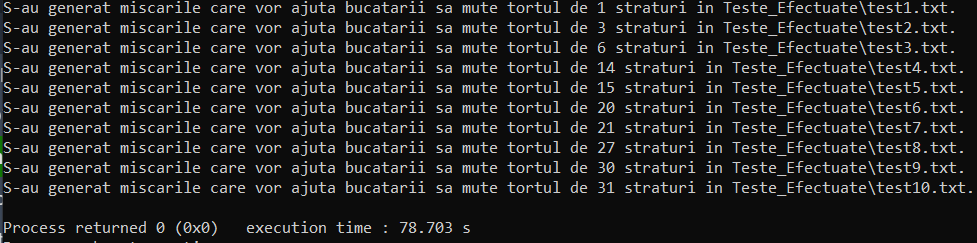
\includegraphics[scale=0.6]{Exemplu_Rulare_Teste}\\

Aceste mesaje vor fi afi'sate pentru oricare dintre cele patru programe.

\newpage

\subsection{Testarea datelor de ie'sire}

Pentru a testa dac'a algoritmul salveaz'a mut'ari corecte 'in fi'sierele de output am folosit mai multe metode:
\begin{itemize}
    \item Pentru valorile mici ale num'arului de straturi am verificat manual mut'arile 'si toate s-au dovedit a fi corecte, iar num'arul de mut'ari salvat de program era cel corect (corespunz"and cu num'arul de mut'ari citite manual).
    \item Pentru valori mai mari, doar am dat scroll prin fi'sier pentru a vedea c'a nu exist'a erori ale mut'arilor (exemplu: nu se muta un strat ce nu apar'tinea intervalului de straturi posibile, acest interval fiind (1,nr\_straturi\_tort), dupa care am verificat num'arul de mutari salvate 'si acesta a fost 'intotdeauna \\
    $2^{nr\_straturi\_tort}-1$, ceea ce 'inseamna c'a a fost calculat corect.
    
    
\end{itemize}


\subsection{Timpii de execu'tie pentru date mici si mari}

Am organizat compararea datelor timpilor de execu'tie 'in dou'a tabele: primul tabel compar'a cele dou'a programe recursive, iar al doilea pe cele dou'a iterative.


\begin{center}

Tabel Comparare Algoritmi Recursivi

\begin{tabular}{|c|c|c|c|}
    \hline
    Nr.Test & Numarul de Straturi & C & Python \\[0.5ex]
    \hline \hline
    1 & 1 & 0.000000 & 0.0 \\
    \hline
    2 & 3 & 0.000000 & 0.0 \\
    \hline
    3 & 6 & 0.000000 & 0.0 \\
    \hline
    4 & 14 & 0.000000 &    0.0069799423217 \\
    \hline
    5 & 15 & 0.000000 &    0.0119671821594  \\
    \hline
    6 & 20 & 0.000000 &    0.3540530204772 \\
    \hline
    7 & 21 & 0.000000 &    0.7011260986328 \\
    \hline
    8 & 27 & 0.000000 &   45.6151285171508 \\
    \hline
    9 & 30 & 2.000000 &  351.2672555446625 \\
    \hline
    10 & 31 & 4.000000 & 749.6825110912323 \\[0.05ex]
    \hline
\end{tabular}

\vspace{\baselineskip}

Tabel Comparare Algoritmi Iterativi

\begin{tabular}{|c|c|c|c|}
    \hline
    Nr.Test & Numarul de Straturi & C & Python \\[0.5ex]
    \hline \hline
    1 & 1 & 0.000000 & 0.0 \\
    \hline
    2 & 3 & 0.000000 & 0.0 \\
    \hline
    3 & 6 & 0.000000 & 0.0 \\
    \hline
    4 & 14 & 0.000000 &      0.019946813583 \\
    \hline
    5 & 15 & 0.000000 &      0.039893150329 \\
    \hline
    6 & 20 & 0.000000 &      1.222729682922 \\
    \hline
    7 & 21 & 0.000000 &      2.431497335433 \\
    \hline
    8 & 27 & 3.000000 &    153.349867105484 \\
    \hline
    9 & 30 & 25.000000 &  1208.827067375183 \\
    \hline
    10 & 31 & 51.000000 & 2403.487896680832 \\[0.05ex]
    \hline
\end{tabular}
\end{center}

\newpage
\subsection{Observa'tii si Concluzii}

Observ'am c'a algoritmii 'in C sunt cu mult mai rapizi decat cei 'in Python, dar observ'am 'si c'a, pentru amblele limbaje, cu c"at numarul de straturi devine mai mare, cu at"at timpul de execu'tie cre'ste.

De asemenea, am observat c'a algoritmul iterativ este mult mai lent dec"at cel recursiv; acest lucru se poate explica prin faptul c'a, pentru algoritmul iterativ am utilizat structuri/liste pentru a crea stive.\\

'In oricare dintre cele patru programe, pentru un set de date de intrare identic, se va ob'tine un set de date de ie'sire identic (pa'sii pentru mutarea tortului), iar num'arul de mut'ari este demonstrat c'a va fi $2^n-1$, unde n reprezint'a num'arul de straturi ale tortului.\\

O parte interesant'a a implement'arii algoritmilor a fost limitarea salv'arilor 'in fi'sier; pe l"ang'a faptul c'a fi'sierul de output c'ap'ata dimensiuni enorme, execu'tia cre'stea mult datorit'a acestor salv'ari. Am ales s'a limitez la 1000 de mut'ari afi'sate algoritmul.

O alt'a parte provocatoare a fost trecerea de la un limbaj compilat la unul interpretat; am studiat, astfel, multe despre limbajul Phyton 'si p"an'a s'a ajung la versiunile finale ale codului, am avut multe alte programe "test" efectuate 'in care am aprofundat utilizarea lui.\\

Pe viitor, acest program poate fi dezvoltat, iar 'in loc s'a afi'seze sau salveze mut'arile efectuate, ar putea s'a le mute grafic 'intr-un program de editare 3D, dar acesta este un proiect de viitor, greu de realizat cu ajutorul cuno'stiin'telor actuale.


\newpage

\begin{thebibliography}{9}

   
    \bibitem{cormen}
     Thomas H. Cormen and Charles E. Leiserson and Ronald L. Rivest and Clifford Stein,
     \emph{Introduction to Algorithms}.
     MIT Press,
     3rd Edition,
     2009.
     
    \bibitem{C}
     Dennis Ritchie and Brian Kernighan,
     \emph{The C Programming Language. 2nd Edition},
     Prentice Hall,
     1978.
     
    \bibitem{Idee}
     \url{https://www.khanacademy.org/computing/computer-science/algorithms/towers-of-hanoi/a/towers-of-hanoi}
     
    \bibitem{latex1}
     \url{https://www.overleaf.com/learn/latex/Learn_LaTeX_in_30_minutes}
     
    \bibitem{latex2}
     \url{https://www.latex-project.org/}
     
    \bibitem{Py}
     \url{https://www.reddit.com/r/Python/}






\end{thebibliography}










\end{document}